\documentclass[tikz,border=12pt]{standalone}
\usepackage[T1]{fontenc}
\usepackage{mathpazo}
\usepackage{amsmath,amssymb}
\usetikzlibrary{arrows.meta, positioning, calc}

\definecolor{stblue}{HTML}{7B97AD}
\definecolor{rwgold}{HTML}{B8995E}
\definecolor{sage}{HTML}{7A9A7E}
\definecolor{dkbrown}{HTML}{3D3530}
\definecolor{wmgray}{HTML}{7B7067}
\definecolor{cream}{HTML}{F9F6F0}
\definecolor{border}{HTML}{D4C9B8}
\definecolor{terracotta}{HTML}{C47A6A}

\begin{document}
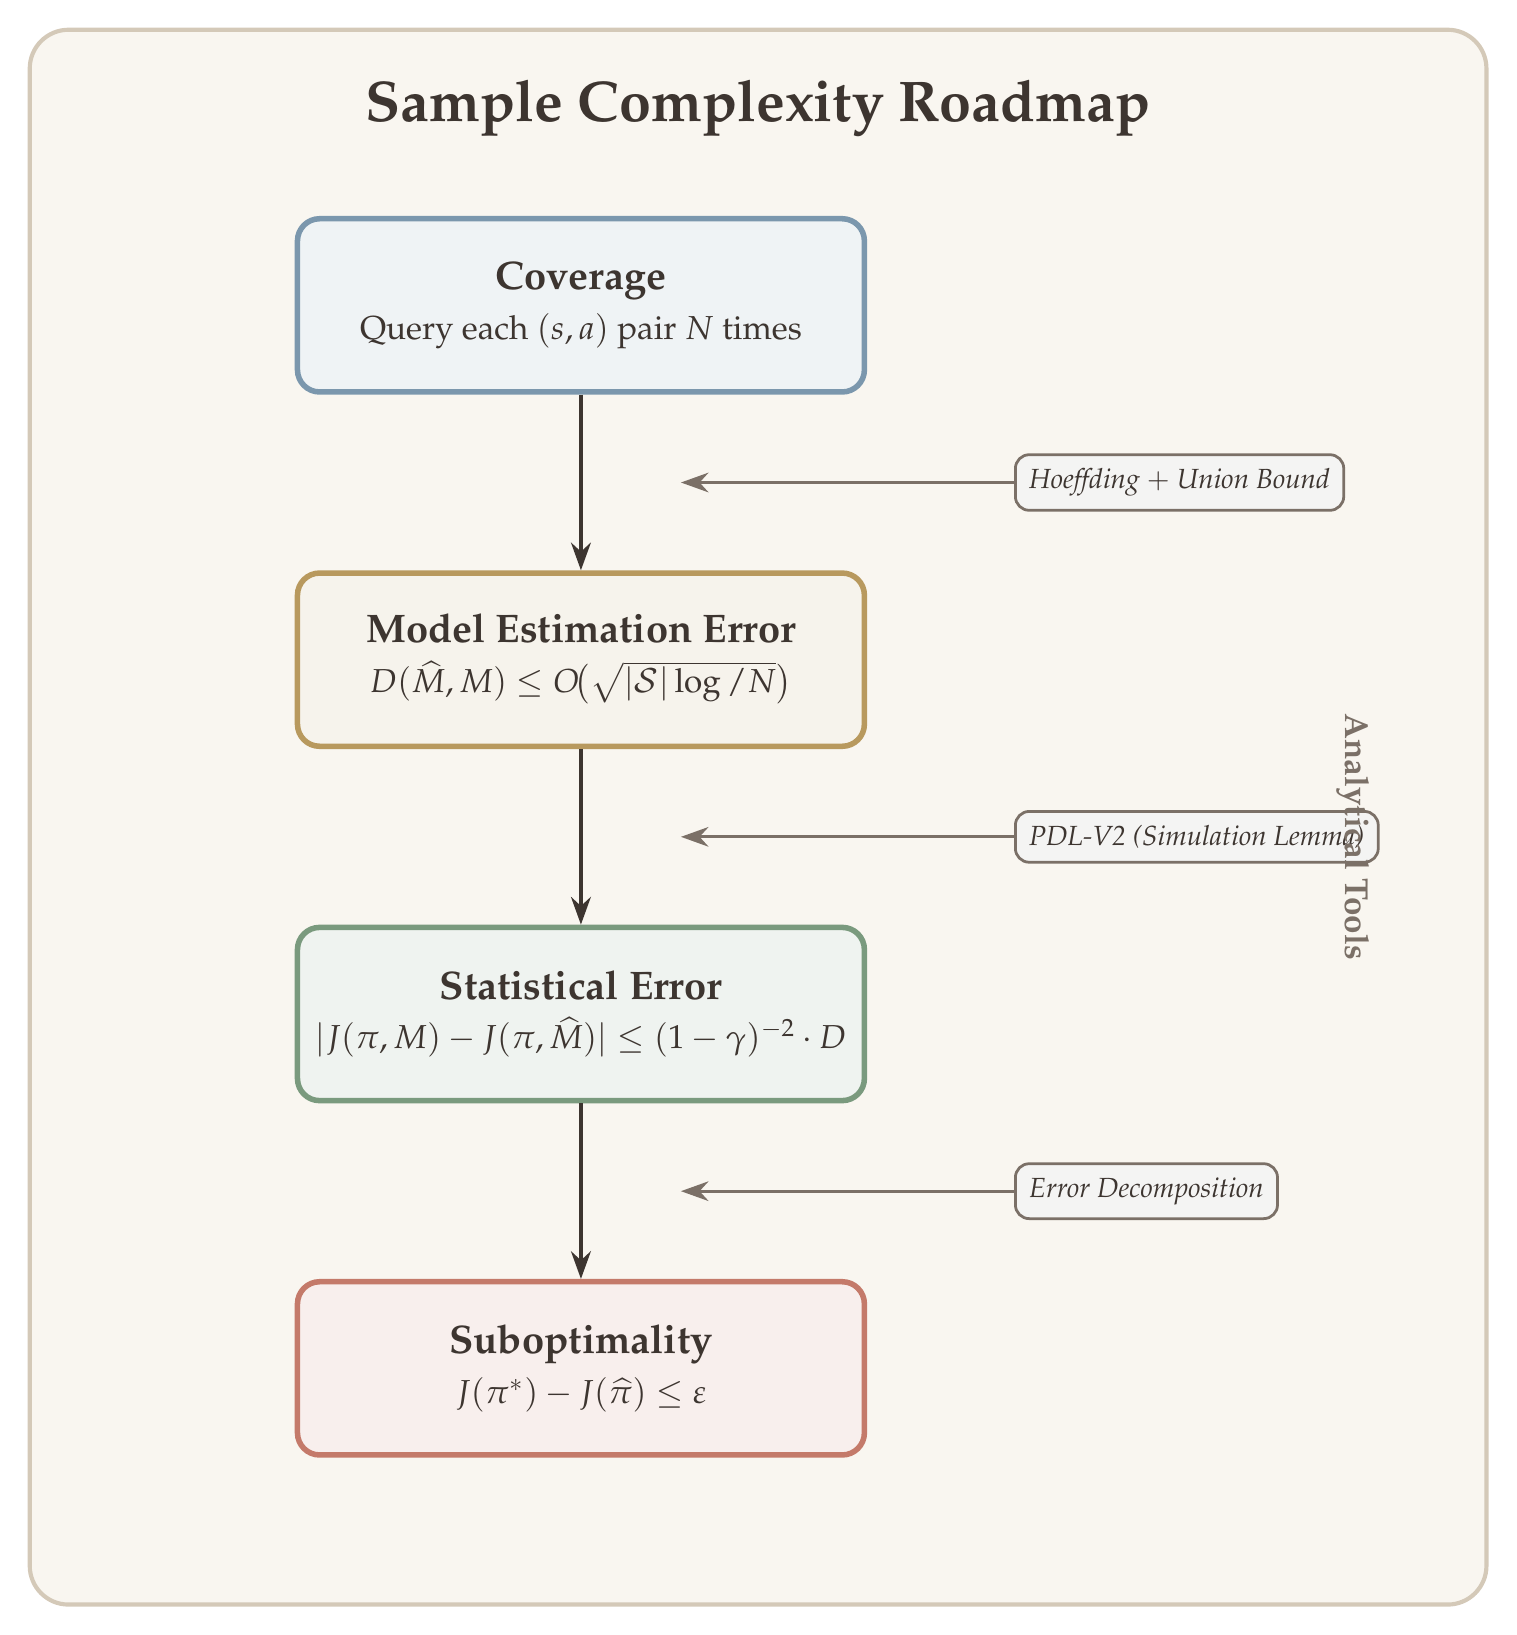
\begin{tikzpicture}[
  >={Stealth[length=3.5mm, width=2.5mm]},
  step/.style={draw=#1, line width=2pt, fill=#1!12, rounded corners=8pt,
    minimum width=72mm, minimum height=22mm, font=\large, text=dkbrown,
    align=center, inner sep=6pt},
  tool/.style={draw=wmgray, line width=1pt, fill=wmgray!8, rounded corners=5pt,
    font=\normalsize\itshape, text=dkbrown, align=center, inner sep=5pt},
  arr/.style={->, line width=1.6pt, dkbrown},
]

% Background
\fill[cream, rounded corners=14pt] (-2.0,-16.5) rectangle (16.5,3.5);
\draw[border, rounded corners=14pt, line width=1.5pt] (-2.0,-16.5) rectangle (16.5,3.5);

% Title
\node[font=\huge\bfseries, text=dkbrown] at (7.25,2.5)
  {Sample Complexity Roadmap};

% =============================================
% Step 1: Coverage
% =============================================
\node[step=stblue] (cov) at (5.0,0.0)
  {\textbf{\Large Coverage}\\[4pt]
   Query each $(s,a)$ pair $N$ times};

% =============================================
% Step 2: Model Estimation Error
% =============================================
\node[step=rwgold] (model) at (5.0,-4.5)
  {\textbf{\Large Model Estimation Error}\\[4pt]
   $D(\widehat{M}, M) \leq O\!\bigl(\sqrt{|\mathcal{S}|\log / N}\bigr)$};

% Arrow 1 -> 2
\draw[arr] (cov.south) -- (model.north);

% =============================================
% Step 3: Statistical Error
% =============================================
\node[step=sage] (stat) at (5.0,-9.0)
  {\textbf{\Large Statistical Error}\\[4pt]
   $|J(\pi, M) - J(\pi, \widehat{M})| \leq (1-\gamma)^{-2} \cdot D$};

% Arrow 2 -> 3
\draw[arr] (model.south) -- (stat.north);

% =============================================
% Step 4: Suboptimality
% =============================================
\node[step=terracotta] (subopt) at (5.0,-13.5)
  {\textbf{\Large Suboptimality}\\[4pt]
   $J(\pi^*) - J(\widehat{\pi}) \leq \varepsilon$};

% Arrow 3 -> 4
\draw[arr] (stat.south) -- (subopt.north);

% =============================================
% Tool annotations (right side)
% =============================================

% Tool 1->2: Hoeffding + Union Bound
\coordinate (mid12) at ($(cov.south)!0.5!(model.north)$);
\node[tool, anchor=west] (t1) at (10.5,-2.25)
  {Hoeffding $+$ Union Bound};
\draw[wmgray, line width=1pt, ->, shorten >=2pt]
  (t1.west) -- ($(mid12) + (1.2,0)$);

% Tool 2->3: PDL-V2 (Simulation Lemma)
\coordinate (mid23) at ($(model.south)!0.5!(stat.north)$);
\node[tool, anchor=west] (t2) at (10.5,-6.75)
  {PDL-V2 (Simulation Lemma)};
\draw[wmgray, line width=1pt, ->, shorten >=2pt]
  (t2.west) -- ($(mid23) + (1.2,0)$);

% Tool 3->4: Error Decomposition
\coordinate (mid34) at ($(stat.south)!0.5!(subopt.north)$);
\node[tool, anchor=west] (t3) at (10.5,-11.25)
  {Error Decomposition};
\draw[wmgray, line width=1pt, ->, shorten >=2pt]
  (t3.west) -- ($(mid34) + (1.2,0)$);

% =============================================
% Vertical "tools" label
% =============================================
\node[font=\large\bfseries, text=wmgray, rotate=-90, anchor=center]
  at (14.8,-6.75) {Analytical Tools};

\end{tikzpicture}
\end{document}
